\chapter{The Dataset}
\label{the_dataset}

% \begin{enumerate}
%     \item The dataset used in this investigation is original, and presents a new opportunity, not seen in the literature thus far.
%     \item In particular it offers a close alignment between features of code, and descriptive elements that aim to tell you the function of the specific code element - distinct from the whole function.
%     \item In this section we will present the means of collection, the structure of the dataset, and finally an analysis of its composition. 
%     \item This analysis aims to be informative by both being quantitative, highlight the statistical composition of the dataset, and qualitative.
%     \item Finally we  also compare it and contrast it to other datasets.
% \end{enumerate}


The dataset used in the our investigation was entirely original, presenting a new opportunity to investigate the machine translation of code not seen in the literature thus far. \textbf{CITE}
In particular it offers a close and granular alignment between elements of code (argument names) and their natural language descriptions, as extracted from the most popular open source Python libraries.
In this section we present first an overview of the dataset, and elaborate on  the means of collection. 
We then present an in-depth analysis of its structure and composition, which aims to be both quantitative, and qualitive, comparing the dataset to others in the field. 

\section{Overview} % (fold)
\label{sec:overview}

The dataset comprises of a list of Python function arguments, their natural language descriptions and surrounding metadata. 
This metadata is extensive, containing numerous fields including the source code of the function, function name and filename, among others. 
The full structure of the data fields is enumerated in Table \ref{table:metadata}. 

This data is sourced exclusively from the top 300 most downloaded libraries on "PyPI", the python package manager. 
This ensured that the libraries were both good quality, well documented, and very much ``real world code.''
The data was then stored in YAML format, for human readability. 
A real example is presented in Appendix \ref{example_datapoint}, Listing \ref{lst:single_point}


\begin{table}[h!]
    \begin{center}
    \begin{tabular}{| c | c | c | c |}
    \hline
        Name &  Description     &    Field    & Type  \\
    \hline
        Argument Name & the name of the argument  & arg\_name & string \\
        Argument Description & the description of the argument & arg\_desc & string \\
        Argument Type & the annotated type for the argument & arg\_type & string or null \\
        All Arguments & all arguments used in the function & args & list of strings \\
        Other Argument Info & name, desc. and type for all other arguments & arg\_info & dict of dicts\\
        Function Name & the name of the function & name & string\\
        Signature & the function signature & sig & string\\
        Path & the full path to the file & filename & string \\
        Library & the library of the function & pkg & string\\
        Source & the source code of the function & src & string\\
        Docstring & the sphinx annotated docstring & docstring & string\\

    \hline


    \end{tabular}
    \caption {Fields collected for each single datapoint. Field refers to the actual key used in YAML file, and Type indicates the type of the data as stored in the file.}
    \label{table:metadata}
    \end{center}
\end{table}


% section overview (end)

\section{Method of Collection} % (fold)
\label{sec:method_of_collection}

\begin{enumerate}
    \item Python is a dynamically typed language, with emphasis on documentation, and naturalness.
    \item Sphinx is the industry standard for automating documentation generation.
    \item It contains an open source plugin `napoleon' that generate html web API documentation for docstrings formatted ether according to the Google Standard or the Numpy Standard (show examples of both).
    \item This appears to be used extensively in industry by xyz
    \item We wrote a plugin forked off napoleon that instead generated parsed the data and wrote it to an output yaml file (CITE)
    \item Since we require libaries with good documentation, that are easy to install (for the plug in to read them - documentation is sources by syntax tree??) we decided to run on the most popular libraries in python. we used the pip wall of superpowers to search for 300 most popular libraries on pip.
    \item After collecting these, we preprocessed by removing arguments without description (ie self), and those without code bodies (Ie (not implemented error) in abstract base class)
    \item more on filtering
\end{enumerate}




\begin{table}[h!]
    \begin{center}
    \begin{tabular}{c | c | c | c}
        Library      & Arguments     & Functions  & Scientific \\
    \hline
        tensorflow   & $ 17002 $     & $ 4340 $ & True \\
        google   & $ 2829 $      & $ 1098 $ & False \\
        scipy    & $ 2030 $      & $ 549 $ & True \\
        networkx     & $ 1869 $      & $ 669 $ & True \\
        matplotlib   & $ 1457 $      & $ 366 $ & True \\
        sklearn      & $ 1403 $      & $ 368 $ & True \\
        pandas   & $ 1317 $      & $ 419 $ & True \\
        magenta      & $ 1045 $      & $ 357 $ & False \\
        (\textit{100 $<$ arguments $<$ 1000})   & $ 10172 $     & $ 3137 $ & True: 6, False: 26 \\
        (\textit{0 $<$ arguments $<$ 100})      & $ 2300 $      & $ 1036 $ & True: 9, False: 84 \\
    \hline
    \hline
        TOTAL    & $ 41424 $     & $ 12339 $ & True: 21, False: 112 \\
    \end{tabular}
    \caption {Break down of the largest libraries in the dataset, by contribution of arguments. Despite their relative infrequency in the overall dataset, scientific libraries contribute the majority of arguments and functions}
    \label{table:breakdown_by_library}
    \end{center}
\end{table}
% section structure_of_dataset (end)

\section{Composition of the Dataset} % (fold)
\label{sec:composition_of_the_dataset}

Although the criteria for choice of library was based solely on frequency of downloads from the Python Package Index, an analysis of the composition of the dataset reveals some biases.
In particular it is clear that scientific libraries are heavily dominate the composition of the data.

Of the 112 libraries that eventually contributed data to the dataset, only 21 are labelled with the `Scientific/Engineering' tag on PYPI, yet these libraries contribute 68.3\% of arguments to the overall dataset, and 61.6\% of the functions. 
Even more surprisingly one library, \mintinline{python}{tensorflow}, contributes 41\% of the arguments to the data - vastly more than any other library.
In fact, as can be seen from Table \ref{table:breakdown_by_library}, it contributes almost six times as many arguments as the second placed library - coincidentally also developed by Google. 

This outsize contribution from relatively few libraries is largely the result of the design of these libraries and their use cases. 
Scientific libraries have vast APIs, and users of the libraries often require different interfaces for potentially similar functions. 
As an example, two library methods such as \mintinline{python}{conv2D} and \mintinline{python}{conv3D} may in an abstract sense perform very similar functions - a mathematical convolution - yet are critically distinct in a scientific setting.
The necessity of these kinds of distinctions, and the precision of their use case, leads these libraries to have large numbers of exposed functions, requiring clear documentation.

The full breakdown of the dataset by library is available on GitHub, alongside the data.

\section{Analysis of Data} % (fold)
\label{sec:analysis_of_data}


\subsection{Statistical Analysis of Natural Language} % (fold)
\label{sub:statistical_analysis_of_natural_language}


\begin{itemize}
    \item Very science heavy (see the variable names \& function names): Table \ref{table:popular_variable_names}
    \item And a lot of repetition of the same variable : Table \ref{table:variable_histogram}
    \item ... and functions Table: \ref{table:function_histogram}
    \item However, these duplicates often have different descriptions, see Table \ref{table:name_desc_histogram}, with examples in Table \ref{table:descriptions_for_names}
    \item ... and also come from different packages in Table \ref{table:packages_for_names}
    \item So in fact the things to worry about are whether enough diversity of package and what is overwhelming the data
    \item in particular look at tensorflow name. 
    \item the average number of functions per argument ($3.836 \pm 2.96$) wo we want a histogram?
    \item The counts of the descriiption lengths and what are the args per function are visible in Fig \ref{fig:seq_length} 
    \item There is evidence to suggest some trimming of data and we do that.

\end{itemize}


\begin{figure}
    \begin{center}
    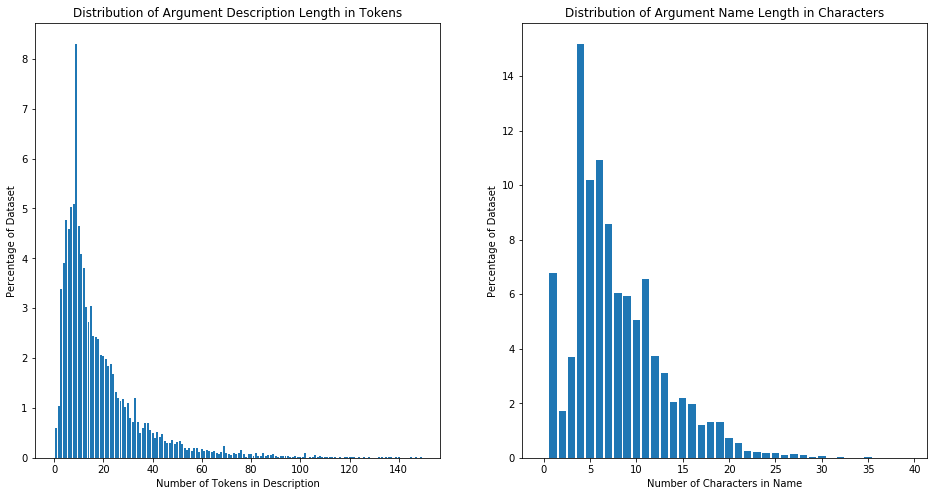
\includegraphics[scale=.5]{SEC4_SequenceLength.png}    
    \end{center}  
        \caption{Histograms of the length of sequences for both argument names and argument descriptions}
    \label{fig:seq_length}
 
\end{figure}
% \begin{enumerate}
%     \item variable name frequencies. TICK
%     \item function name frequencies. TICK
%     \item description lengths  TICK   !!
%     \item duplicates       TICK
%     \item tf-idf
%     \item arg per funcion CROSS
% \end{enumerate}

\begin{table}[h!]
    \begin{center}
    \begin{tabular}{c | c | c | c | c}
    & Top Argument Names & Count  &   Top Function Names & Count \\  
    \hline               
    1.   &  name     &     1917    &   fit       &    122 \\        
    2.   &  x        &     439     &   transform &    102 \\         
    3.   &  kwargs   &     303     &   train     &    77 \\         
    4.   &  axis     &     263     &   evaluate  &    71 \\        
    5.   &  dtype    &     260     &   get       &    61 \\         
    6.   &  a        &     230     &   conv2d    &    59 \\        
    7.   &  G        &     227     &   Client    &    52 \\        
    8.   &  inputs   &     224     &   update    &    46 \\        
    9.   &  input    &     223     &   add       &    45 \\         
    10.  &  value    &     210     &   specgram  &    45 \\         
    
    \end{tabular}
    \caption {The most popular variable names and function names in the raw dataset. As can be seen these are either dominated by scientific terms and single letter variable names, such as those in scientific libraries. Scientific functions which take large numbers of arguments contribute heavily to the dataset}
    \label{table:popular_variable_names}
    \end{center}
\end{table}

\begin{table}[p]
    \begin{center}
    \begin{tabular}{c | c | c | c  }       
     Bin   & \multicolumn{3}{c}{Counts of Variable Name}   \\
    \hline
     &     raw &... as \% of unique names & ... as \% of all names   \\  
    \hline     
     1     &      3681 &   53.550 &   11.738  \\          
     2 - 4 &      2141 &   31.146 &   17.302  \\          
     5 - 9 &       539 &    7.841 &   10.989  \\          
     10 - 19 &     272 &    3.957 &   11.464  \\          
     20 - 99 &     212 &    3.084 &   26.122  \\          
     100 - 499 &    28 &    0.407 &   16.272  \\          
     500 - 1999 &    1 &    0.015 &    6.113  \\                

    \end{tabular}
        \caption { A table of the count and frequency of variable names as they feature in the raw dataset. Approximately half of all variables names occur over 10 times in the data. In particular a single outlier - the variable name \mintinline{python}{name} from \mintinline{python}{tensorflow}, accounts for 6.1\% of the collected data}
    \label{table:variable_histogram}

    \begin{tabular}{c | c | c | c  }       

     Bin   & \multicolumn{3}{c}{Counts of Variable (Name, Description) Pairs}  \\
    \hline
     &     raw &... as \% of unique pairs & ... as \% of all pairs  \\  
    \hline     
    1 &     14956 &   77.009 &   47.691  \\
    2 - 4 &      3799 &   19.561 &   28.881 \\
    5 - 9 &       480 &    2.472 &    9.483 \\
    10 - 99 &     185 &    0.953 &   10.574 \\
    100 - 499 &     0 &    0.000 &    0.000 \\
    500 - 1999 &    1 &    0.005 &    3.371 \\           

    \end{tabular}
        \caption { A table of the count and frequency of function names as they feature in the dataset. Although names are often repeated, a much greater fraction of data points have unique (name, description) pairs.}
    \label{table:name_desc_histogram}

    %% TO DO: Function names & argument sizes, not just "name" 
    \begin{tabular}{c | c | c | c  }       
     Bin   & \multicolumn{3}{c}{Counts of Variable Function Name}   \\
    \hline
     &     raw &... as \% of unique names & ... as \% of all names   \\  
    \hline     
    1   &      2453 &   28.774 &    7.822  \\          
    2 - 4 &      3946 &   46.287 &   34.324  \\          
    5 - 9 &      1649 &   19.343 &   32.930  \\          
    10 - 19 &     384 &    4.504 &   15.523  \\          
    20 - 99 &      91 &    1.067 &    8.686  \\          
    100 - 499 &     2 &    0.023 &    0.714  \\          
    500 - 1999 &    0 &    0.000 &    0.000  \\             

    \end{tabular}
        \caption { A table of the count and frequency of function names of the variables as they feature in the raw dataset. 
        These can be either due to the repetition of function name throughout libraries, or by one argument contributing many functions }
    \label{table:function_histogram} 
    \end{center}
\end{table}



\subsection{Statistical Analysis of Code} % (fold)
\label{sub:statistical_analysis_of_code}

\begin{enumerate}
    \item Very few paths are unique, which is unsurprising given the abstractness and simplicity of the Python syntax tree
    \item However, each point has many many paths.  about half are between 50 and 500 paths.
    \item  Some functions have preposterous large numbers of paths due to the fact that the variable is is referred to multiple times in the code, and large class definitions. 
    \item This is very much like a real word dataset, where syntax trees are significant and varried
\end{enumerate}





\begin{table}[p]

    \begin{tabular}{c | c | c}       
    
    & Most Popular Paths  &  \% of Data \\  
   \hline
                
1.  & Name $\leftarrow$ keyword $\leftarrow$ Call $\rightarrow$ keyword &  0.679 \\ 
2.  & Name $\leftarrow$ Call $\rightarrow$ Name &  0.672 \\ 
3.  & Name $\leftarrow$ keyword $\leftarrow$ Call $\rightarrow$ keyword $\rightarrow$ Name &  0.647 \\ 
4.  & Name $\leftarrow$ Call $\rightarrow$ Attribute &  0.296 \\ 
5.  & Name $\leftarrow$ Call $\rightarrow$ Attribute $\rightarrow$ Name &  0.241 \\ 
6.  & Name $\leftarrow$ keyword $\leftarrow$ Call $\leftarrow$ Assign $\leftarrow$ If $\rightarrow$ Assign $\rightarrow$ Name &  0.229 \\ 
7.  & Name $\leftarrow$ AugAssign $\leftarrow$ For $\leftarrow$ FunctionDef $\rightarrow$ Assign $\rightarrow$ List $\rightarrow$ List $\rightarrow$ Num &  0.210 \\ 
8.  & Name $\leftarrow$ keyword $\leftarrow$ Call $\leftarrow$ Assign $\leftarrow$ If $\rightarrow$ Try $\rightarrow$ Assign $\rightarrow$ Call $\rightarrow$ Name &  0.192 \\ 
9.  & Name $\leftarrow$ Call $\leftarrow$ Assign $\leftarrow$ Try $\leftarrow$ If $\rightarrow$ Assign $\rightarrow$ Name &  0.189 \\ 
10.  & Name $\leftarrow$ Call $\leftarrow$ Assign $\leftarrow$ Try $\leftarrow$ If $\rightarrow$ Assign $\rightarrow$ Call $\rightarrow$ keyword &  0.184 \\ 
  
  \end{tabular}
      \caption { The most popular the paths of the the dataset. These only account for a very small amount of the data }
    \label{table:function_histogram} 
    \begin{center}
    \begin{tabular}{c | c | c | c c }       
        Occurences Bin   & \multicolumn{3}{c}{Counts of Code Paths}   \\
        \hline
         &     raw &... as \% of unique paths & ... as \% of all paths   \\  
        \hline     
        1 &     229107 &   33.753 &    2.195  \\                                       
        2 - 9 &     346845 &   51.099 &   12.056  \\                                       
        10 - 99 &   91261 &   13.445 &   22.349  \\                                        
        100 - 999 & 10247 &    1.510 &   26.367    \\                                      
        1000 - 9999 & 1280 &    0.189 &   30.418  \\                                       
        10000 - 99999 &   37 &    0.005 &    6.615   \\                                 
                                                                     
    \end{tabular}
        \caption { A table of the count and codepaths as they feature in the raw dataset. A larfe fraction of the datasets are repeated }
    \label{table:function_histogram} 
    \begin{tabular}{c | c | c  }       
    
   Paths Per DataPoint & Count  &  \%-ile of data points \\  
   \hline
    0 &               24  &     0.07865 \\
    1 &               138  &    0.53090 \\
    2 - 9 &           2451  &   8.56328 \\
    10 - 49 &         8717  &   37.13050 \\
    50 - 99 &         4517  &   51.93354 \\
    100 - 499 &       10023  &  84.78076 \\
    500 - 999 &       2449  &   92.80658 \\
    1000 - 9999 &     2160  &   99.88530 \\
    10000 - 99999 &   32  &     99.99017 \\
    100000 - 999999 & 3  &      100.00000 \\

  \end{tabular}
    \caption { A table of the count and frequency of distinct code paths as they feature in the raw dataset. 
        These can be either due to the repetition of function name throughout libraries, or by one argument contributing many functions }
    \label{table:function_histogram} 

    \end{center}
\end{table}










% subsection statistical_analysis_of_code (end)

\subsection{Qualitative Analysis of Dataset} % (fold)
\label{sub:qualitative_analysis_}
So far looked at frequencies and seen that some argument sharing between similar libraries, but how different are diffrenet libraries on a description level?


tfidf \& tsne


\section{Final Preparations} % (fold)
\label{sec:final_preparations}

A table of the final datasets used in the experiment (duplicates filtered or not, split vs unsplit)


% subsection qualitative_analysis_ (end)
% section analysis_of_data (end)

\subsection{Comparison To Other Datasets} % (fold)
\label{sub:comparison_to_other_datasets}

    This should be contrasted with comments, and overall docstrings, and full annotations.
    \begin{itemize}
        \item Comments data set - often comment is extra information when reading code. Why - not what
        \item Docstrings - have much more context and can be unspecific. It is unclear what partof the code does what. The mapping is very unclear
        \item Annotations - much more granular and good mapping of meaning to description, but not organic necessarily. DIfficult to source large dataset in.
    \end{itemize}




% subsection comparison_to_other_datasets (end)